\section{Ενισχυτής Σφάλματος}\label{section:EA}

Ο ενισχυτής σφάλματος (error amplifier) θα υλοποιηθεί με ένα nMOS διαφορικό ζεύγος εισόδου με ενεργό φορτίο $\symup{P}_3$ και $\symup{P}_4$ όπως φαίνεται στο σχήμα \ref{fig:error_amplifier:schematic}. Λαμβάνεται απλή έξοδος από την πλευρά του $\symup{N}_2$. Στην σχεδίαση συμπεριλαμβάνονται και τα $\symup{N}_5$ και $\symup{N}_6$, μέρος του κυκλώματος πόλωσης. Αρχικά, στην υποενότητα \ref{subsection:ea:ratios} γίνεται μία εκτίμηση των λόγων των transistor επιβάλλοντας κάποιες προδιαγραφές. Έπειτα, στην υποενότητα \ref{subsection:ea:sim} αναφέρονται οι τροποποιήσεις που έγιναν και παρουσιάζονται οι προσομοιώσεις που πραγματοποιήθηκαν. Τέλος, στην υποενότητα \ref{subsection:ea:layout} παρατίθεται και σχολιάζεται το φυσικό σχέδιο του ενισχυτή.

\begin{figure}[h!]
	\centering
	\begin{tikzpicture}
	% Paths, nodes and wires:
	\node[pigfete, solderdot, xscale=-1](pMOS3) at (-1.5, 3){} node[anchor=east] at (pMOS3.text){$\symup{P}_{3}$};
	\node[pigfete, solderdot](pMOS4) at (1.5, 3){} node[anchor=west] at (pMOS4.text){$\symup{P}_{4}$};
	\draw (-1.5, 2.23) -| (-1.5, 0.77);
	\draw (1.5, 0.77) -| (1.5, 2.23);
	\draw (-0.52, 3.27) -- (0.52, 3.27);
	\draw (-0.52, 3.27) |- (-1.5, 2.23);
	\node[circ, xscale=-0.75, yscale=0.75] at (-0.52, 3.27){};
	\node[circ, xscale=-0.75, yscale=0.75](N1) at (-1.5, 2.23){} node[anchor=east] at (N1.east){$E$};
	\node[vcc](VDD) at (-1.5, 3.77){} node[anchor=south] at (VDD.text){$V_{DD}$};
	\node[vcc](N2) at (1.5, 3.77){} node[anchor=south] at (N2.text){$V_{DD}$};
	\draw (-1.5, -0.77) -| (-1.5, -1) -- (1.5, -1) -| (1.5, -0.77);
	\draw (2.75, 2) to[capacitor, l={$C_{\symup{load}}$}] (2.75, 1);
	\node[tlground] at (2.75, 1){};
	\draw (1.5, 2) -- (4, 2);
	\node[circ, xscale=0.75, yscale=0.75] at (2.75, 2){};
	\node[ocirc](N3) at (4, 2){} node[anchor=west] at (N3.east){$v_{\symup{out}}$};
	\node[circ, xscale=0.75, yscale=0.75] at (0, -1){};
	\node[tlground] at (0, -2.54){};
	\draw (-3.02, -2.04) -- (-0.98, -2.04);
	\draw (-4, -1) -| (-3.02, -2.04);
	\node[circ, xscale=0.75, yscale=0.75] at (-3.02, -2.04){};
	\node[circ, xscale=0.75, yscale=0.75] at (-4, -1){};
	\node[tlground] at (-4, -2.54){};
	\draw (-4, 1) to[american current source, l_={$I_{\symup{bias}}$}] (-4, -1);
	\node[vcc](N4) at (-4, 1){} node[anchor=south] at (N4.text){$V_{DD}$};
	\node[circ, xscale=0.75, yscale=0.75] at (1.5, 2){};
	\node[nigfete, solderdot](nMOS5) at (0, -1.77){} node[anchor=west] at (nMOS5.text){$\symup{N}_{5}$};
	\node[nigfete, solderdot, xscale=-1](nMOS6) at (-4, -1.77){} node[anchor=east] at (nMOS6.text){$\symup{N}_{6}$};
	\node[nigfetebulk, xscale=-1](nMOS2) at (1.5, -0){} node[anchor=south east] at ([xshift=-0.32cm, yshift=0.32cm]nMOS2.west){$\symup{N}_{2}$};
	\draw (1.5, -0) -| (1.167, -0.333);
	\node[tlground] at (1.167, -0.333){};
	\node[nigfetebulk](nMOS1) at (-1.5, -0){} node[anchor=south west] at ([xshift=0.32cm, yshift=0.32cm]nMOS1.west){$\symup{N}_{1}$};
	\node[tlground] at (-1.167, -0.333){};
	\draw (-1.5, -0) -| (-1.167, -0.333);
	\node[ocirc](vin2) at (2.48, -0.27){} node[anchor=west] at (vin2.east){$v_{\symup{in}2}$};
	\node[ocirc](vin1) at (-2.48, -0.27){} node[anchor=east] at (vin1.west){$v_{\symup{in}1}$};
\end{tikzpicture}
	\caption{Σχηματικό ενισχυτή σφάλματος. Αποτελείται από ένα διαφορικό nMOS ζεύγος, $\symup{N}_1$ και $\symup{N}_2$, ενεργό φορτίο pMOS, $\symup{P}_3$ και $\symup{P}_4$, με το $\symup{P}_3$ σε συνδεσμολογία διόδου και τον καθρέπτη ρεύματος, $\symup{N}_5$ και $\symup{N}_6$. Οδηγεί, στην έξοδο, χωρητικό φορτίο, $C_{\symup{load}}$.}
	\label{fig:error_amplifier:schematic}
\end{figure}

\subsection{Εκτίμηση των Λόγων των Transistor}\label{subsection:ea:ratios}

Η συνάρτηση μεταφοράς του ενισχυτή του σχήματος \ref{fig:error_amplifier:schematic} δίνεται από την εξίσωση \eqref{eq:error_amplifier:transfer_function} \cite{RazaviCMOS}.

\begin{equation}
	\label{eq:error_amplifier:transfer_function}
	H(s)=\symcal{L}\left[\frac{v_{\symup{out}}}{v_{\symup{in}}}\right](s)=\frac{A_0 \left( 2 + \displaystyle\frac{s}{\omega_{p2}} \right)}{\left( 1 + \displaystyle\frac{s}{\omega_{p1}} \right) \left( 1 + \displaystyle\frac{s}{\omega_{p2}} \right)},
\end{equation}
όπου $A_0$ είναι το dc κέρδος και $\omega_{p1}$, $\omega_{p2}$ είναι οι δύο πόλοι της $H$. Το dc κέρδος είναι \cite{RazaviCMOS}
\begin{equation*}
	A_0=g_{mn}\left(r_{on}\parallel r_{op}\right)=g_{mn}\frac{r_{on} r_{op}}{r_{on}+r_{op}}.
\end{equation*}

Ο πρώτος πόλος οφείλεται στο μονοπάτι $\symup{N}_1 \to \symup{P}_3 \to  \symup{P}_4$ \cite{RazaviCMOS} και δίνεται προσεγγιστικά από την έκφραση
\begin{equation}
	\label{eq:error_amplifier:pole1}
	\omega_{p1}\approxeq \left[ \left(r_{on}\parallel r_{op}\right) C_{\symup{load}} \right]^{-1}=\frac{r_{on}+r_{op}}{r_{on} r_{op} C_{\symup{load}}}.
\end{equation}
Ο δεύτερος πόλος οφείλεται στο μονοπάτι $\symup{N}_1 \to \symup{Ν}_2$ \cite{RazaviCMOS} και δίνεται προσεγγιστικά από την έκφραση
\begin{equation}
	\label{eq:error_amplifier:pole2}
	\omega_{p2}\approxeq \frac{g_{mp}}{C_E},
\end{equation}
όπου $C_E$ είναι η ισοδύναμη χωρητικότητα στον κόμβο $E$ προς τη γείωση. Η ισοδύναμη χωρητικότητα οφείλεται, μεταξύ άλλων, στις παρασιτικές χωρητικότητες $C_{gs3}$, $C_{gs4}$, στο φαινόμενο Miller των $C_{gd1}$ και $C_{gd4}$ \cite{RazaviCMOS}.\par
Επιπλέον, η \eqref{eq:error_amplifier:transfer_function} παρουσιάζει μηδενικό στη συχνότητα $\omega_z=\nicefrac{2 g_{mp}}{C_E}=2\omega_{p2}$.\par
Ο ενισχυτής θα οδηγεί την πύλη του $\symup{M_{pe}}$, όπως φαίνεται στο σχήμα \ref{fig:LDO:schematic}. Λόγω του μεγάλου μεγέθους του $\symup{M_{pe}}$, η χωρητικότητα φορτίου του ενισχυτή σφάλματος μπορεί να θεωρηθεί επαρκώς μεγαλύτερη των παρασιτικών χωρητικοτήτων των transistor του ενισχυτή. Επομένως, για απλούστευση των υπολογισμών, θεωρούμε πως στον κόμβο $E$ κυριαρχεί η χωρητικότητα φορτίου, $C_{\symup{load}}$.\par
Έστω πως απαιτούμε συχνότητα μοναδιαίου κέρδους $f_{u}=5\unit{\mega\hertz}$, dc κέρδος $A_0=5\unit{\volt\per{\volt}}$, μέγιστη χωρητικότητα φορτίου $\max{\left(C_{\symup{load}}\right)}=25\unit{\pico\farad}$
% περιθώριο φάσης $\symup{PM}=60\unit{\degree}$ \cite{ChenPower}
και ρυθμό μεταβολής εξόδου (slew rate) $\symup{SR}=10\unit{\volt\per{\micro\second}}$.\par
% Το περιθώριο φάσης (phase margin) υπολογίζεται από την εξίσωση \eqref{eq:error_amplifier:phase_margin}. Είναι θεμιτό η συχνότητα μοναδιαίου κέρδους, $f_{u}$ ή $\omega_{u}$, να είναι μικρότερη του μηδενικού, $\omega_{z}$, και του δεύτερου πόλου, $\omega_{p2}$, \cite{SedraSmith}. Θέτουμε $\omega_z=10\omega_{u}=20\pi f_{u}$. Επιπλέον, θεωρούμε πως, λόγω της μεγάλης χωρητικότητας φορτίου, η συχνότητα του πρώτου πόλου τείνει στο μηδέν, $\omega_{p1}\to 0$.
% \begin{equation}
% 	\label{eq:error_amplifier:phase_margin}
% 	\symup{PM}=180\unit{\degree}-\left[ \arctan{\left( \frac{\omega_{u}}{\omega_{p1}} \right)} + \arctan{\left( \frac{\omega_{u}}{\omega_{p2}} \right)} + \arctan{\left( \frac{\omega_{u}}{\omega_{z}} \right)}\right]
% \end{equation}

% Εφαρμόζοντας τις παραπάνω παραδοχές στην εξίσωση \eqref{eq:error_amplifier:phase_margin} προκύπτει $\omega_{p2}\geqq 2.216\omega_{u}$ ή ισοδύναμα --λόγω της \eqref{eq:error_amplifier:pole2} και της υπόθεσης $C_E\approxeq C_{\symup{load}}$-- η διαγωγιμότητα των $\symup{P}_3$ και $\symup{P}_4$ πρέπει να πληροί την συνθήκη $g_{mp}\geqq 2.216\omega_{u} C_{\symup{load}}$.\par
Για τα ρεύματα των transistor $\symup{N}_1$, $\symup{N}_2$, $\symup{P}_3$, $\symup{P}_4$ και $\symup{N}_5$ ισχύει $i_{d5}=2i_{di},\forall i\in\left[1,4\right]$ \cite{RazaviFundamentals}. Το $i_{d5}$ προσδιορίζεται μέσω του ρυθμού μεταβολής εξόδου: $i_{d5}=\symup{SR}\cdot C_{\symup{load}}$. Θεωρώντας τα $\symup{P}_3$ και $\symup{P}_4$ στην περιοχή κορεσμού μπορούμε να υπολογίσουμε τον λόγο τους, $S=\nicefrac{W}{L}$, (αγνοώντας την διαμόρφωση καναλιού) μέσω της \eqref{eq:error_amplifier:pMOS_saturation_current} \cite{SedraSmith}.
\begin{equation}
	\label{eq:error_amplifier:pMOS_saturation_current}
	i_{d3}=i_{d4}=\frac{1}{2}k_{p}^{\prime}S_{3}\left( v_{sg3} - \left|V_{th,p}\right| \right)^2,
\end{equation}
όπου $v_{sg3}=V_{DD}-\max{\left( v_{\symup{in}} \right)}+V_{th,n}$ θεωρώντας πως τα $\symup{N}_1$ και $\symup{N}_2$ λειτουργούν στην περιοχή κορεσμού ($v_{gd}\leqq V_{th,n}$ \cite{SedraSmith}). Επομένως, το πλάτος, $W$, των transistor $\symup{P}_3$ και $\symup{P}_4$ δίνεται από την έκφραση \eqref{eq:error_amplifier:W34}.
\begin{equation}
	\label{eq:error_amplifier:W34}
	W_{3}=W_{4}=L\frac{i_{d5}}{k_{p}^{\prime} \left[ V_{DD}-\max{\left( v_{\symup{in}} \right)}+V_{th,n}-\left|V_{th,p}\right| \right]^2},
\end{equation}
όπου $L$ το μήκος του καναλιού.\par
Η διαγωγιμότητα των transistor $\symup{N}_1$ και $\symup{N}_2$ μπορεί να υπολογιστεί μέσω της συχνότητας μοναδιαίου κέρδους. Θα είναι $\omega_{u}=A_0\omega_{p1}$ \cite{SedraSmith}. Δηλαδή, προκύπτει για τα $\symup{N}_1$ και $\symup{N}_2$: $g_{mn}=2\pi f_{u}C_{\symup{load}}$. Η έκφραση του ρεύματος στον κορεσμό είναι
\begin{equation}
	i_{d1}=i_{d2}=\frac{g_{mn}^{2}}{2k_{n}^{\prime}S_{1}}.
\end{equation}
Επομένως, το μήκος των το πλάτος, $W$, των transistor $\symup{N}_1$ και $\symup{N}_2$ δίνεται από την έκφραση \eqref{eq:error_amplifier:W12}.
\begin{equation}
	\label{eq:error_amplifier:W12}
	W_1=W_2=L\frac{g_{mn}^{2}}{k_{n}^{\prime}i_{d5}}.
\end{equation}

Τέλος, ο λόγος του transistor $\symup{N}_5$ (λειτουργεί στην περιοχή κορεσμού) δίνεται από την \eqref{eq:error_amplifier:W5}.
\begin{equation}
	\label{eq:error_amplifier:W5}
	W_5=L\frac{2i_{d5}}{k_{n}^{\prime}v_{ds5,\symup{sat}}^{2}},
\end{equation}
όπου
\begin{equation*}
	v_{ds5,\symup{sat}}=\min{\left( v_{\symup{in}} \right)}-\sqrt{\frac{i_{d5}}{k_{n}^{\prime}S_1}}-V_{th,n}.
\end{equation*}

Για την εκτίμηση της τιμή της παραμέτρου διαγωγιμότητας, $k^{\prime}$, και της τάσης κατωφλίου, $V_{th}$, τα transistor προσομοιώθηκαν στην περιοχή κορεσμού με δύο διαφορετικές διαφορές δυναμικού πύλης-πηγής, $v_{sg}$. Στην πρώτη προσομοίωση ήταν $\left|V_{sg}\right|=1\unit{\volt}$ και στην δεύτερη ήταν $\left|V_{sg}\right|=0.9\unit{\volt}$. Αγνοώντας το φαινόμενο διαμόρφωσης καναλιού, η τάση κατωφλίου εκτιμάται μέσω της σχέσης \eqref{eq:Vth_estimation}.
\begin{equation}
	\label{eq:Vth_estimation}
	\left|V_{th}\right|=\frac{V_{sg}-\sqrt{\nicefrac{I_{ds,1\unit{V}}}{I_{ds,900\unit{\milli\volt}}}}}{1-\sqrt{\nicefrac{I_{ds,1\unit{V}}}{I_{ds,900\unit{\milli\volt}}}}}
\end{equation}
Έχοντας την εκτίμηση της τάσης κατωφλίου, η παράμετρος διαγωγιμότητας είναι
\begin{equation}
	k^{\prime}=2I_{ds}\cdot\left[ \frac{W}{L}\left(V_{sg}-\left|V_{th}\right|\right)^2 \right]^{-1}
\end{equation}

Έτσι, για τα nMOS \texttt{nmos2v} προκύπτει $V_{th,n}=0.35542\unit{\volt}$ και $k_{n}^{\prime}=9.9336\symup{E}-5 \unit{\ampere\per{\volt\squared}}$. Για τα pMOS \texttt{pMOS2v} προκύπτει $V_{th,p}=-0.25710\unit{\volt}$ και $k_{p}^{\prime}=6.4448\symup{E}-5 \unit{\ampere\per{\volt\squared}}$. Οι τιμές αυτές δεν είναι σταθερές, αλλάζουν βάσει της συνδεσμολογίας των ακροδεκτών, του μεγέθους των συσκευών και άλλων φαινομένων που δεν έχουν ληφθεί υπόψιν.\par
Οι εκτιμήσεις για τα μεγέθη του transistor, βάσει των παραπάνω, συνοψίζονται στον πίνακα \ref{table:ratios:estimate}. Το μήκος όλων των transistor είναι το ελάχιστο δυνατό, $L=150\unit{\nano\meter}$. Το $I_{d5}$ προέκυψε $250\unit{\micro\ampere}$.\par

\begin{table}[h!]
\centering
\begin{tabular}{lllllll}
	\specialrule{.1em}{.05em}{.05em}
	& $\symbfup{N_{1}}$ & $\symbfup{N_{2}}$ & $\symbfup{P_{3}}$ & $\symbfup{P_{4}}$ & $\symbfup{N_{5}}$ & $\symbfup{N_{6}}$ \\ \hline
	\multicolumn{1}{l}{$\symbfit{W}\ (\unit{\micro\meter})$} & $3.725841$      & $3.725841$      & $2.343177$      & $2.343177$      & $25.01529$      &  $25.01529$     \\ \hline
	\multicolumn{1}{l}{$\symbfit{L}\ (\unit{\nano\meter})$}  & $150$           & $150$           & $150$           & $150$           & $150$           & $150$           \\ \hline
	\multicolumn{1}{l}{$\symbfit{S}$}                        & $24.83894$      & $24.83894$      & $15.62118$      & $15.62118$      & $ 166.7686$     & $ 166.7686$     \\ \specialrule{.1em}{.05em}{.05em}
\end{tabular}
\caption{Εκτιμώμενο μήκος καναλιού $(L)$, πλάτος $(W)$ και λόγος $S=\nicefrac{W}{L}$ για τα transistor του ενισχυτή σφάλματος.}
\label{table:ratios:estimate}
\end{table}

\subsection{Προσομοιώσεις}\label{subsection:ea:sim}
% Simulations
Στην παρούσα ενότητα παρουσιάζονται τα αποτελέσματα των προσομοιώσεων (AC και Transient Analysis) για τον χαρακτηρισμό της συμπεριφοράς του κυκλώματος. Τα αποτελέσματα επαληθεύονται βάσει της θεωρητικής ανάλυσης απόκρισης συχνότητας ενισχυτών CMOS.

\begin{figure}[h!]
	\centering
	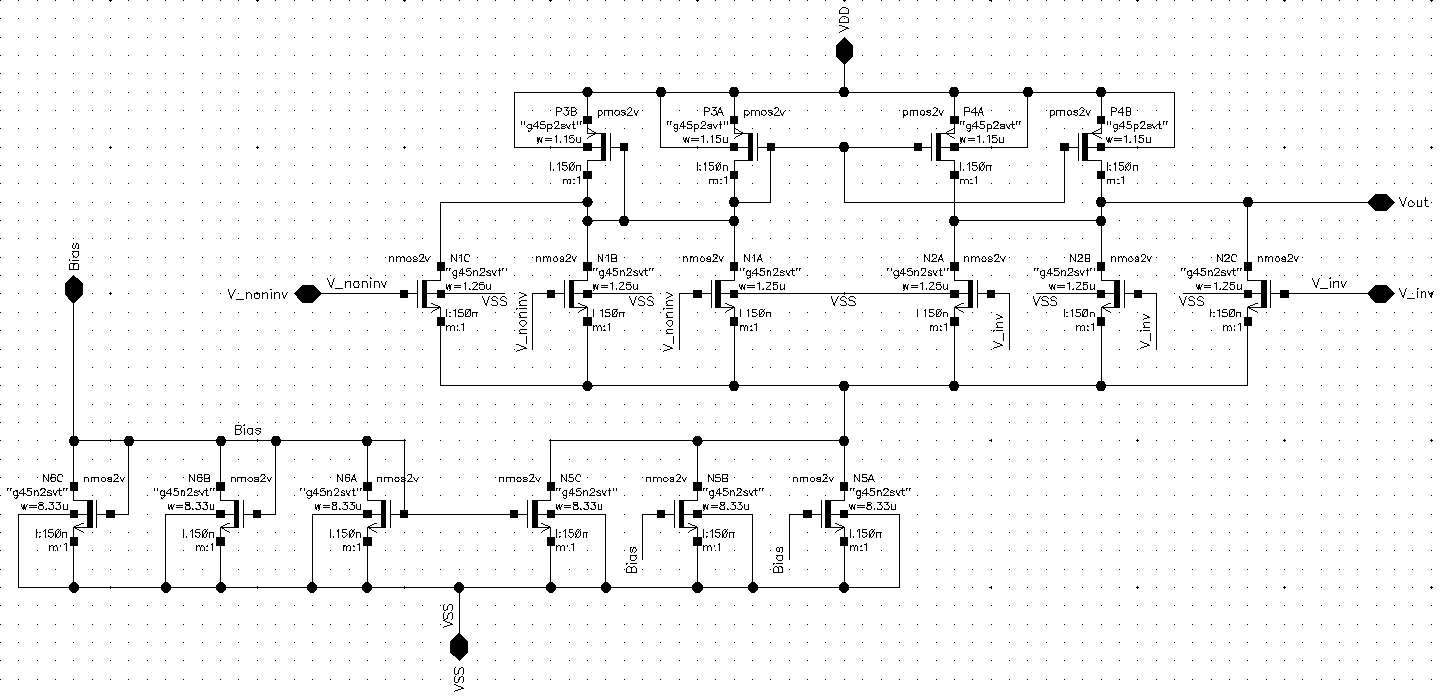
\includegraphics[width=0.75\textwidth]{assets/virtuoso/schematics/Error_Amplifier_Schematic_Final.png}
	\caption{Σχηματικό του ενισχυτή σφάλματος που χρησιμοποιήθηκε για τις προσομοιώσεις και για το φυσικό σχέδιο.}
	\label{fig:error_amplifier_schematic_virtuoso}
\end{figure}


% Bandwidth
\subsubsection{Εύρος Ζώνης}

Η απόκριση συχνότητας του ενισχυτή παρουσιάζεται στο Σχήμα \ref{fig:bandwidth}. Παρατηρούμε ότι το κέρδος τάσης παραμένει σταθερό στις χαμηλές συχνότητες, γεγονός που αντιστοιχεί στο DC κέρδος ($A_0$) της διάταξης, ενώ η πτώση του κέρδους στις υψηλές συχνότητες ακολουθεί τη χαρακτηριστική συμπεριφορά συστήματος δύο πόλων \cite{RazaviCMOS}.

Το εύρος ζώνης $-3\unit{\decibel}$ ($\symup{BW}$) μετρήθηκε στα $1.71\unit{\mega\hertz}$. Η τιμή αυτή προσδιορίζεται στο σημείο όπου το κέρδος τάσης μειώνεται στο $70.7\%$ (ή $-3\unit{\decibel}$) της μέγιστης τιμής του, επαληθεύοντας τον τυπικό ορισμό της συχνότητας $\omega_{-3\unit{\decibel}}$ για αναλογικά κυκλώματα, όπως ορίζεται στη σχέση $\left\|H(j\omega)\right\| = \nicefrac{A_0}{\sqrt{2}}$ \cite{RazaviCMOS}. Η συχνότητα μοναδιαίου κέρδους, $\omega_{u}\colon 20\log{H(s_{u})}=0\unit{\decibel}$, είναι πάνω από $100\unit{\mega\hertz}$ με το δίκτυο ανάδρασης του σχήματος \ref{fig:bandwidth}.\par

\begin{figure}[H]
	\centering
	
\includegraphics[width=0.8\linewidth]{assets/virtuoso/graphs/bandwidth.pdf}
	\caption{Διάγραμμα απόκρισης συχνότητας (AC Analysis). Το εύρος ζώνης -3dB εντοπίζεται στη συχνότητα των $1.71\unit{\mega\hertz}$.}
	\label{fig:bandwidth}
\end{figure}

\begin{figure}[h]
	\centering
	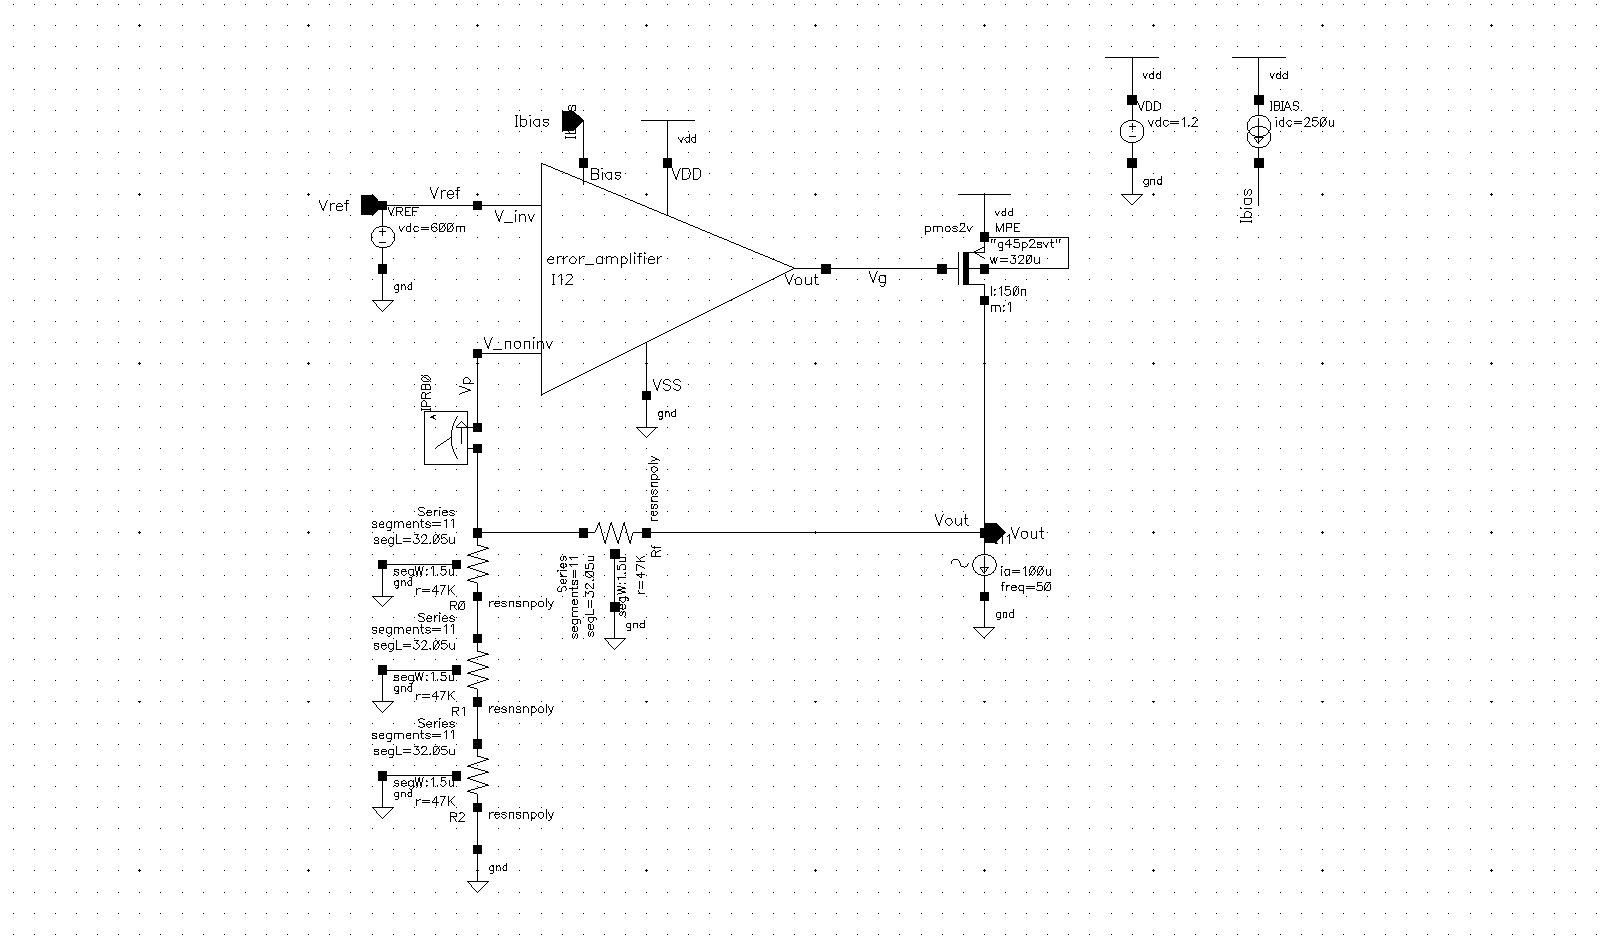
\includegraphics[width=0.8\linewidth]{assets/virtuoso/schematics/testbenches/bandwidth_tb.png}
	\caption{Το σχηματικό που χρησιμοποιήθηκε για την εύρεση του εύρους ζώνης.}
	\label{fig:bandwidth_schematic}
\end{figure}

% Slew Rate
\subsubsection{Ρυθμός Μεταβολής}

Η μεταβατική απόκριση του κυκλώματος σε βηματική είσοδο απεικονίζεται στο Σχήμα \ref{fig:slew_rate}. Η ανάλυση αυτή είναι κρίσιμη για τον προσδιορισμό της ταχύτητας με την οποία η έξοδος μπορεί να ακολουθήσει απότομες μεταβολές της εισόδου.\par

Όπως φαίνεται στο διάγραμμα, η τάση εξόδου ανέρχεται ομαλά χωρίς έντονα φαινόμενα υπερύψωσης (overshoot), γεγονός που υποδηλώνει ευσταθή συμπεριφορά. Ο ρυθμός μεταβολής τάσης (Slew Rate) υπολογίστηκε από την κλίση της καμπύλης για τα σημεία που αντιστοιχούν στην ανύψωση από 10\% έως 90\%, και βρέθηκε ίσος με $41\unit{\volt\per{\micro\second}}$.\par

\begin{figure}[H]
	\centering
	
\includegraphics[width=0.8\linewidth]{assets/virtuoso/graphs/slew_rate.pdf}
	\caption{Μεταβατική απόκριση (Transient Response) σε βηματική είσοδο. Ο ρυθμός μεταβολής (Slew Rate) υπολογίστηκε στα $41\unit{\volt\per{\micro\second}}$.}
	\label{fig:slew_rate}
\end{figure}

\begin{figure}[h]
	\centering
	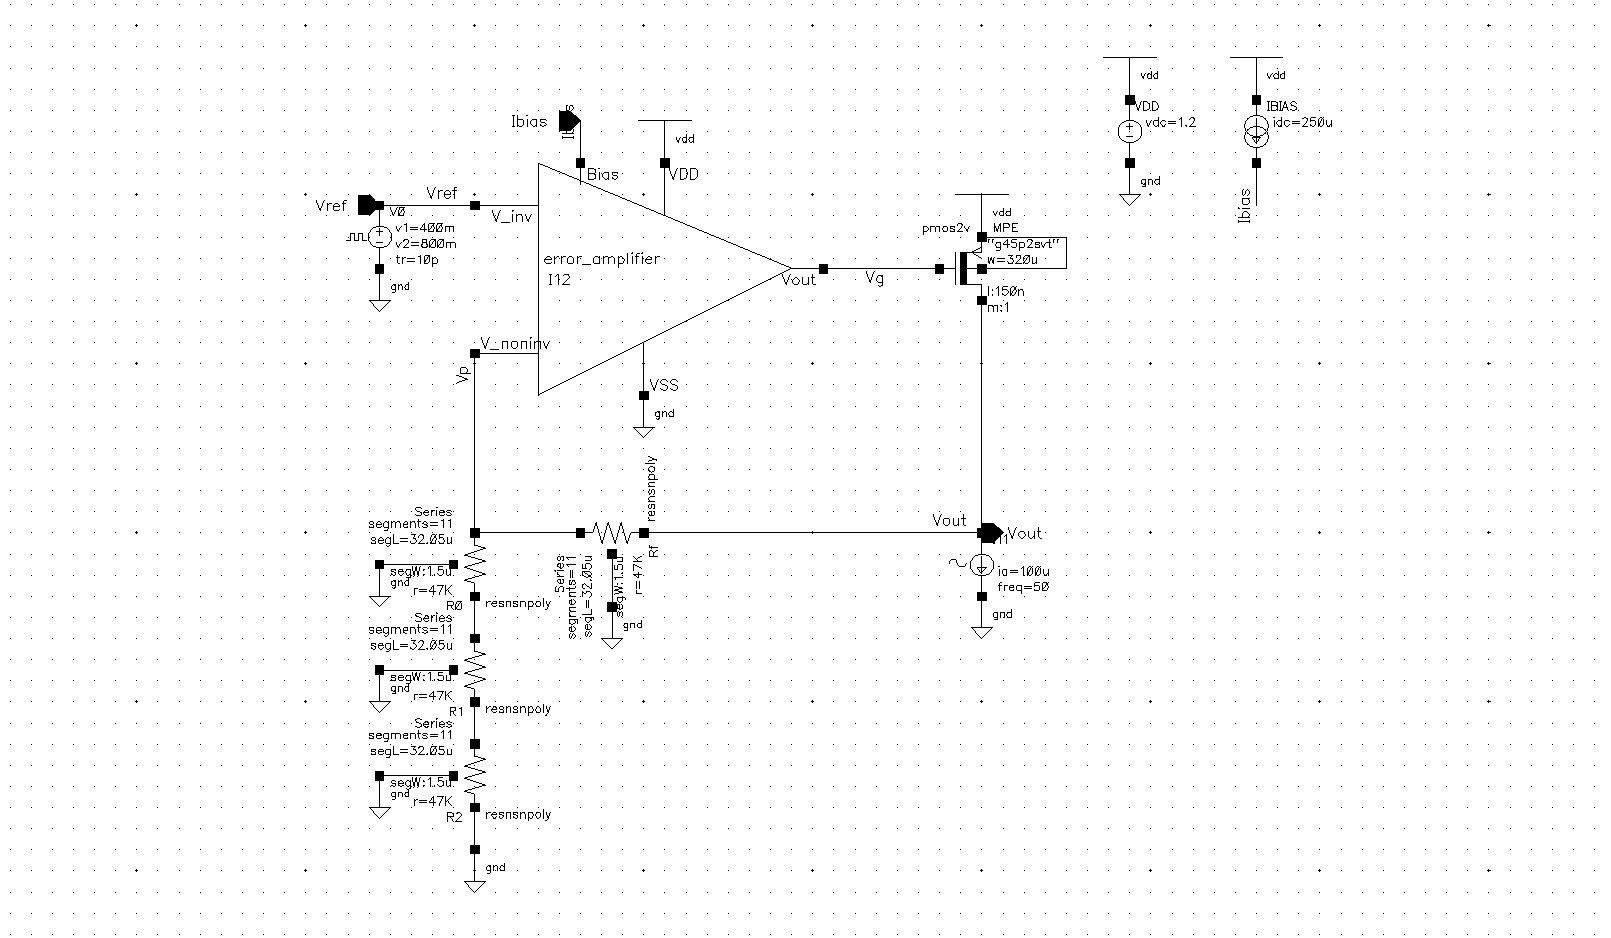
\includegraphics[width=0.8\linewidth]{assets/virtuoso/schematics/testbenches/slewrate_tb.png}
	\caption{Το σχηματικό που χρησιμοποιήθηκε για την εύρεση του ρυθμού μεταβολής.}
	\label{fig:slew_rate_schematic}
\end{figure}


% Gain & Phase
\subsubsection{Απόκριση Κέρδους και Φάσης}

Το Σχήμα \ref{fig:gain_phase} παρουσιάζει το συνδυαστικό διάγραμμα Bode για το μέτρο του κέρδους και το περιθώριο φάσης μέσω ανάλυσης ευστάθειας (\texttt{stb}). Όσον αφορά το κέρδος τάσης, παρατηρούμε ότι στις χαμηλές συχνότητες (DC) διατηρεί μια σταθερή μέγιστη τιμή, η οποία μετρήθηκε στα $49.7\unit{\decibel}$, πριν αρχίσει να μειώνεται μετά τη συχνότητα αποκοπής.\par
Το περιθώριο φάσης ξεκινάει, περίπου, από τις $150\unit{\degree}$ και μειώνεται με την αύξηση της συχνότητας. Στην συχνότητα μοναδιαίου κέρδους, το περιθώριο φάσης είναι $79.55\unit{\degree}\gneqq 45\unit{\degree}$. Επομένως, το σύστημα είναι ικανοποιητικά ευσταθές και είναι δύσκολη η εκκίνηση ταλάντωσης. Η καμπύλη του περιθωρίου φάσης, και συνεπώς της φάσης της εξόδου, ομοιάζει της χαρακτηριστικής καμπύλης συστημάτων δύο πόλων \cite{RazaviCMOS}.\par
% Η συμπεριφορά αυτή είναι συνεπής με τη θεωρητική προσέγγιση Miller για την απόκριση συχνότητας, όπου η κυρίαρχη χωρητικότητα στον κόμβο εξόδου ή στον κόμβο υψηλής αντίστασης καθορίζει την πτώση της φάσης \cite{RazaviCMOS}.\par

\begin{figure}[H]
	\centering
	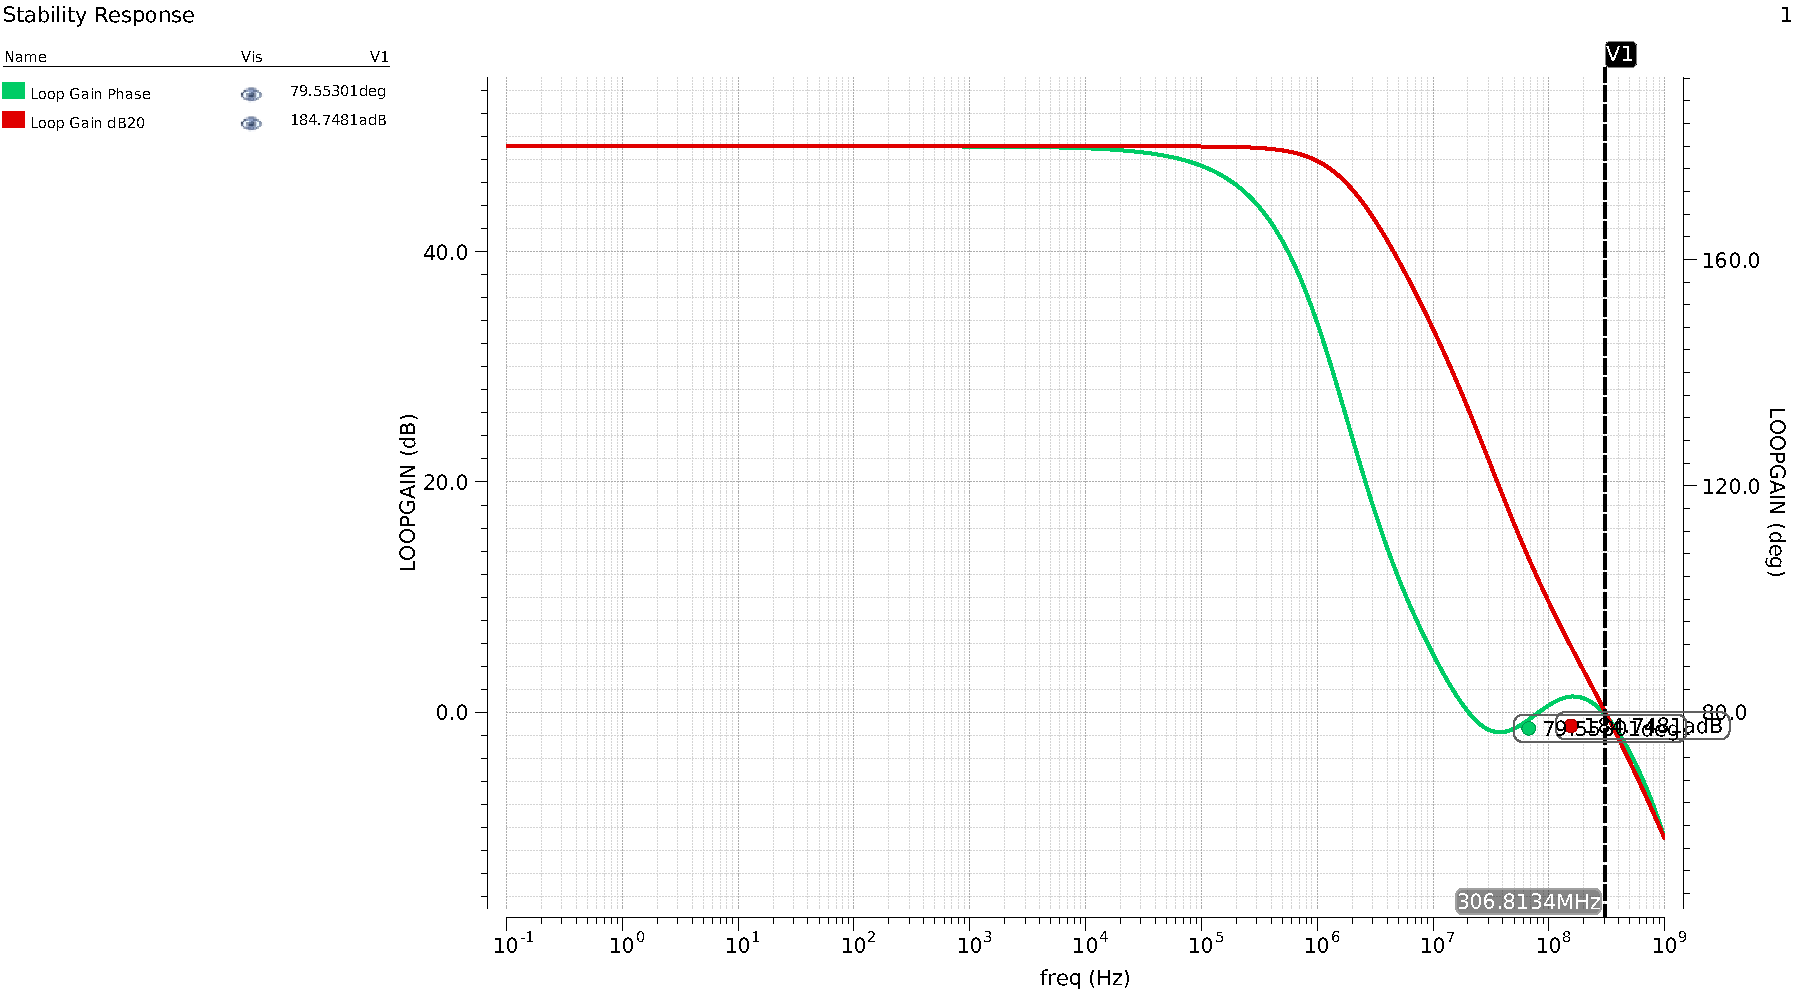
\includegraphics[width=0.8\linewidth]{assets/virtuoso/graphs/gain_phase.pdf}
	\caption{Διάγραμμα Bode κέρδους και περιθωρίου φάσης. Η πτώση της φάσης ακολουθεί τη θεωρητική πρόβλεψη κυρίαρχου πόλου.}
	\label{fig:gain_phase}
\end{figure}

\begin{figure}[h]
	\centering
	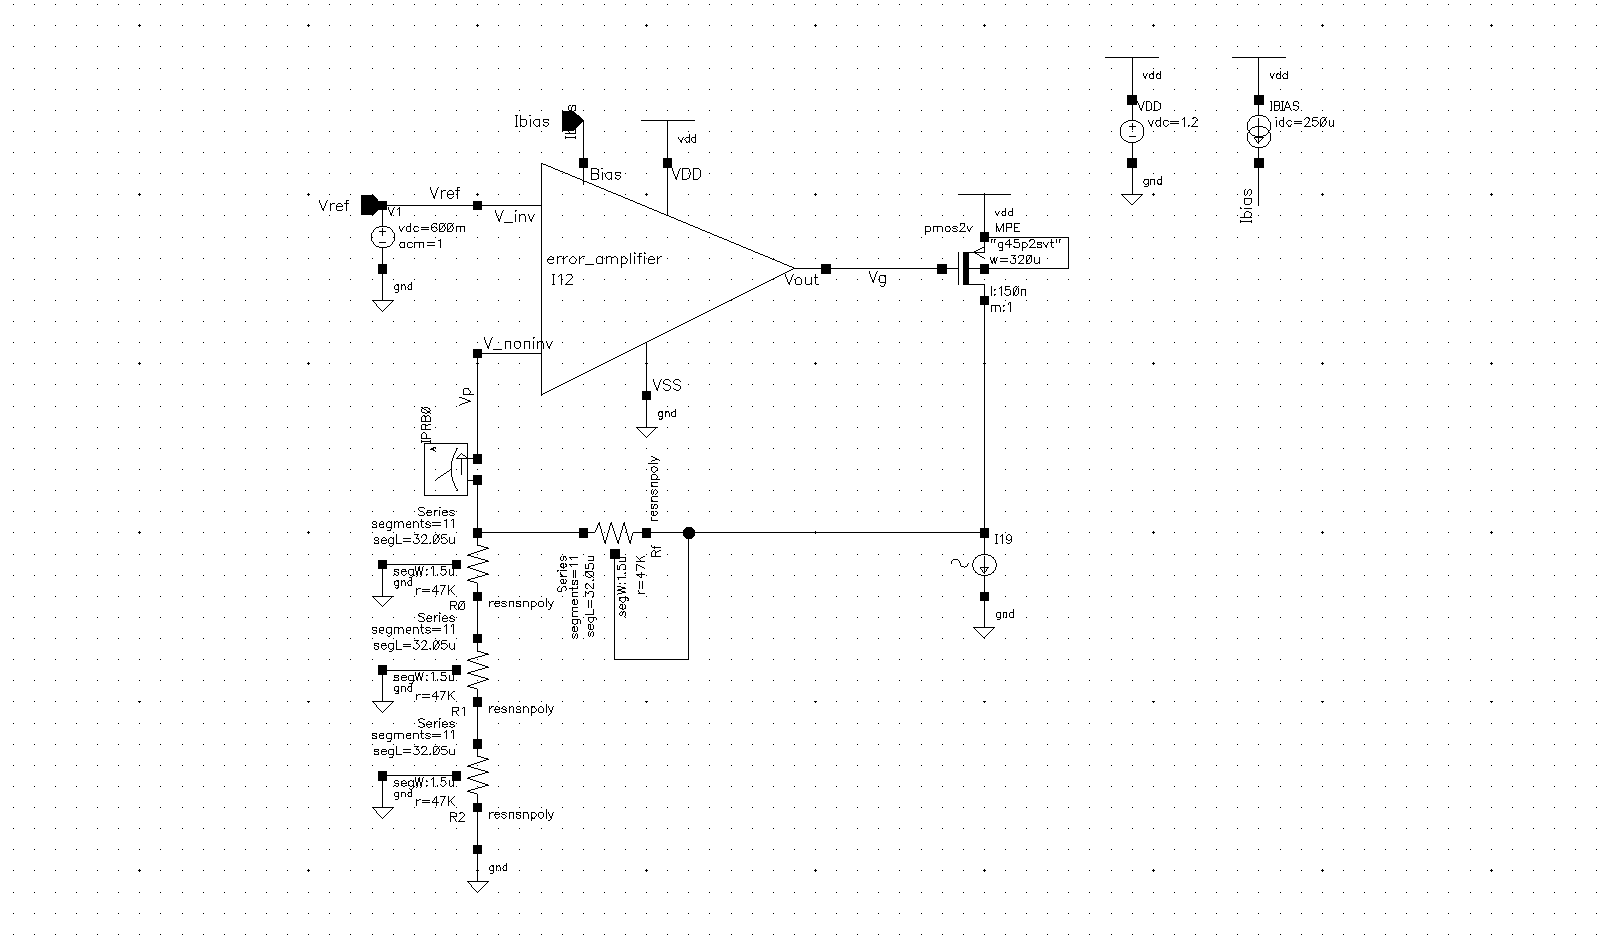
\includegraphics[width=0.8\linewidth]{assets/virtuoso/schematics/testbenches/dc_gain_tb.png}
	\caption{Το σχηματικό που χρησιμοποιήθηκε για την εύρεση του κέρδους.}
	\label{fig:gain_phase_schematic}
\end{figure}

% == Layout == %
\subsection{Φυσικό Σχέδιο}\label{subsection:ea:layout}

Το σχηματικό βάσει του οποίου πραγματοποιήθηκε το φυσικό σχέδιο φαίνεται στο σχήμα \ref{fig:error_amplifier_schematic_virtuoso}. Για τις κατακόρυφες διασυνδέσεις έχουν επιλεχθεί μέταλλα άρτιου αναγνωριστικού αριθμού/επιπέδου και για τις οριζόντιες έχουν επιλεχθεί μέταλλα περιττού αναγνωριστικού αριθμού/επιπέδου. Εξαίρεση της σύμβασης αυτής αποτελεί το δίκτυο \texttt{net59} που συνδέει την εκροή του $\symup{N}_{1}$ με την εκροή και την πύλη του $\symup{P}_3$ και την πύλη του $\symup{P}_4$.\par
Κάθε transistor του σχήματος \ref{fig:error_amplifier:schematic} έχει επιμεριστεί σε μικρότερα transistors με ίδιο μήκος καναλιού και δύο fingers με πλάτος τέτοιο, ώστε το συνολικό πλάτος να μένει σταθερό. Αυτό επιτρέπει την  τοποθέτηση των ταιριασμένων transistor με κοινές τις περιοχές της πηγής όπως φαίνεται στο σχήμα \ref{fig:diff_pair_layout}. Σε κάθε τμήμα του επιμερισμένου transistor τα ρεύματα εκροής-πηγής είναι αντίρροπα. Η μεθοδολογία αυτή μειώνει την πιθανότητα τα transistor να μην είναι ταιριασμένα \cite{Maloberti} και εφαρμόζεται στο διαφορικό ζεύγος $\symup{N}_1$-$\symup{N}_2$ και στα ζεύγη των καθρεπτών ρεύματος $\symup{N}_5$-$\symup{N}_6$ και $\symup{P}_3$-$\symup{P}_4$.\par
Το φυσικό σχέδιο του ενισχυτή σφάλματος φαίνεται στο σχήμα \ref{fig:error_amplifier_layout}. Αριστερά είναι τοποθετημένα τα transistor $\symup{N}_{5x}$-$\symup{N}_{6x}$. Δεξιά πάνω είναι τοποθετημένα τα transistor $\symup{P}_{3x}$-$\symup{P}_{4x}$ και κάτω δεξιά είναι τοποθετημένο το διαφορικό ζεύγος $\symup{N}_{1x}$-$\symup{N}_{2x}$. Πάνω αριστερά έχει τοποθετηθεί η θετική τροφοδοσία $V_{DD}$ και η διεπαφή με το κύκλωμα πόλωσης (bias). Κάτω αριστερά είναι τοποθετημένη η αρνητική τροφοδοσία $V_{SS}$. Πάνω δεξιά έχει τοποθετηθεί η έξοδος του ενισχυτή $v_{\symup{out}}$ και κάτω δεξιά είναι τοποθετημένες οι μη αναστρέφουσα είσοδος και αναστρέφουσα είσοδος, $v_{\symup{in1}}$ και $v_{\symup{in2}}$, αντιστοίχως.\par
Τα nMOS στοιχεία περιβάλλονται από guard ring το οποίο πολώνει το p υπόστρωμα εφαρμόζοντας το δυναμικό $V_{SS}$. Τα pMOS στοιχεία περιβάλλονται από δύο guard rings. Το έσω guard ring πολώνει το πηγάδι τύπου n εφαρμόζοντας δυναμικό $V_{DD}$ και το έξω guard ring εξασφαλίζει πως το p υπόστρωμα βρίσκεται σε χαμηλό δυναμικό εξασφαλίζοντας την ανάστροφη πόλωση της pn επαφής που δημιουργείται μεταξύ υποστρώματος p και πηγαδιού n.\par
\begin{figure}[h!]
	\centering
	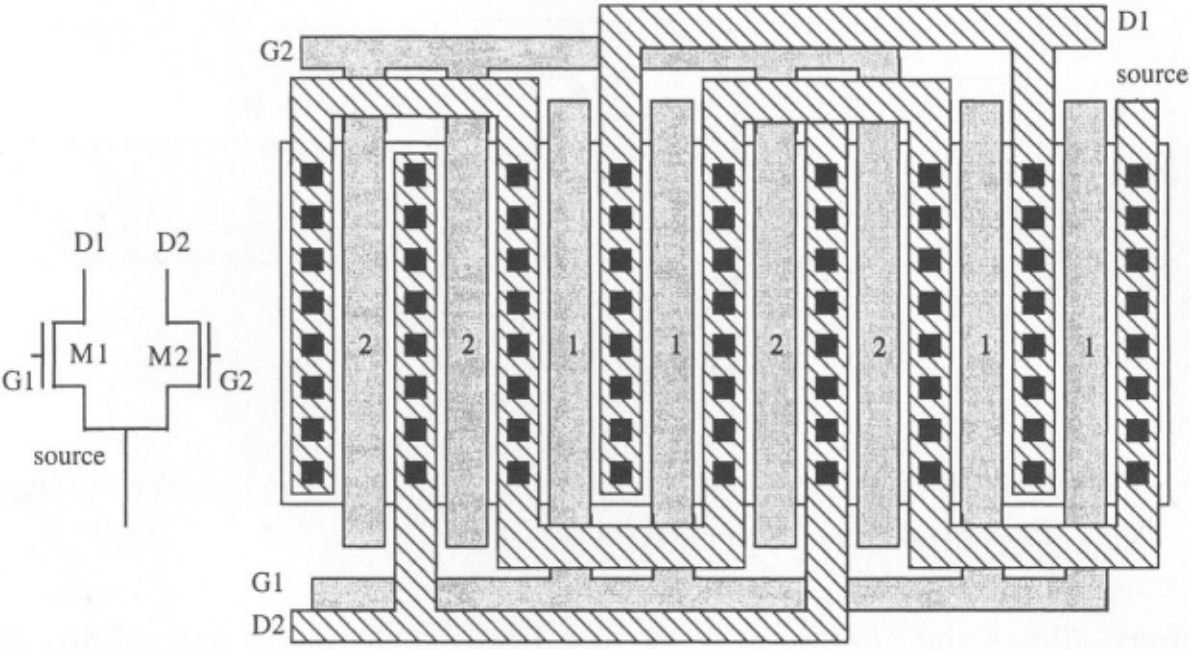
\includegraphics[width=0.75\textwidth]{assets/virtuoso/layout/diff_pair.png}
	\caption{Φυσικό σχέδιο διαφορικού ζεύγους transistor με κοινή πηγή. Πηγή \cite{Maloberti}.}
	\label{fig:diff_pair_layout}
\end{figure}

\begin{figure}[h!]
	\centering
	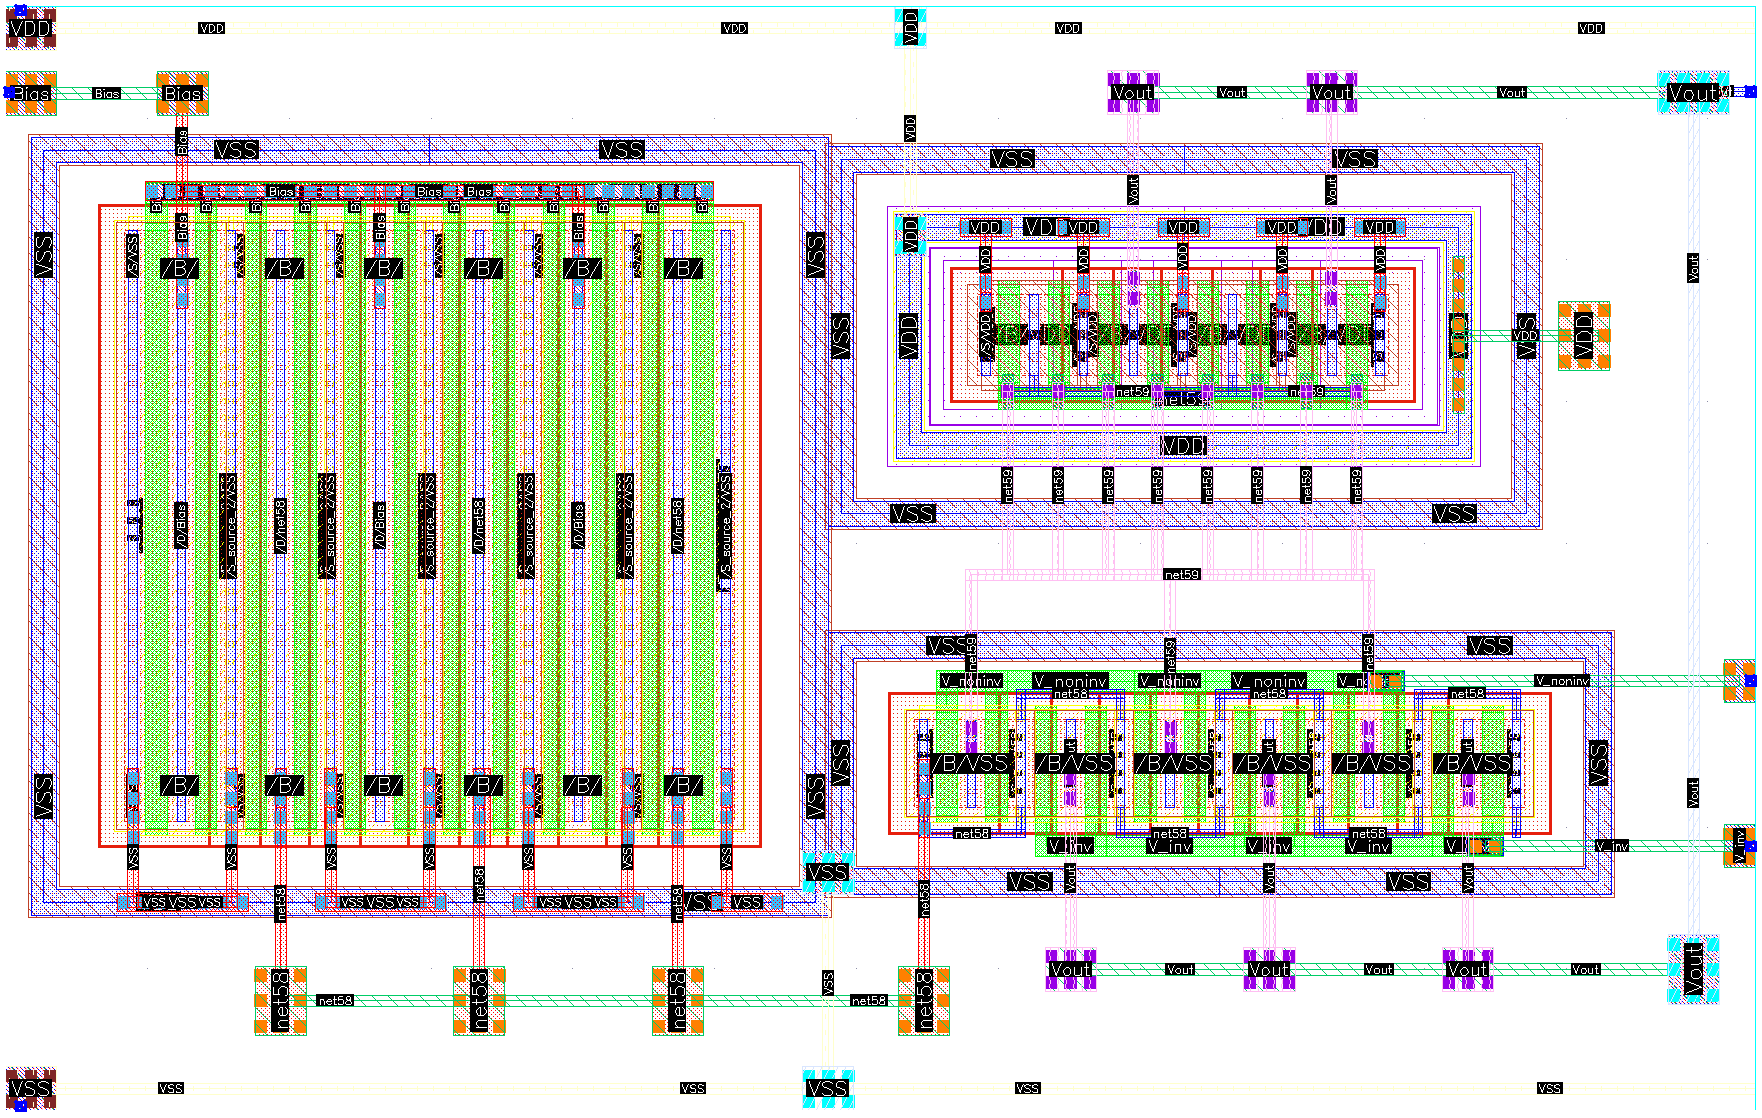
\includegraphics[width=1\textwidth]{assets/virtuoso/layout/ERROR_AMPLIFIER_LAYOUT_2x.png}
	\caption{Φυσικό σχέδιο του ενισχυτή σφάλματος. Αριστερά: $\symup{N}_{5x}$-$\symup{N}_{6x}$. Δεξιά πάνω: $\symup{P}_{3x}$-$\symup{P}_{4x}$. Δεξιά κάτω: $\symup{N}_{1x}$-$\symup{N}_{2x}$. Στο σχήμα \ref{fig:error_amplifier:layout_black} το φυσικό σχέδιο παρατίθεται σε μαύρο φόντο.}
	\label{fig:error_amplifier_layout}
\end{figure}

Πραγματοποιήθηκε dc προσομοίωση για την εύρεση των dc ρευμάτων. Ο αριθμός των vias επιλέχθηκε έτσι, ώστε --βάσει των ρευματικών πυκνοτήτων που αναφέρονται στο εγχειρίδιο της τεχνολογίας-- να υπάρχει περιθώριο υποστήριξης ρευμάτων μεγαλύτερων αυτών της dc προσομοίωσης.\par
Το φυσικό σχέδιο του σχήματος \ref{fig:error_amplifier_layout} πέρασε επιτυχώς τους ελέγχους DRC (design rule check) και LVS (layout versus schematic) όπως φαίνεται στο σχήμα \ref{fig:error_amplifier:layout_DRC_LVS} του παραρτήματος \ref{appendix:layout}.\par
Ελλείψει χρόνου κάποιοι συμβιβασμοί ήταν αναπόφευκτοι. Το φυσικό σχέδιο επιδέχεται βελτιώσεων όπως η χρήση dummy transistors προκειμένου τα ακραία τμήματα των transistor να μην έχουν διαφορετικές παραμέτρους από τα εσωτερικά τμήματα \cite{Maloberti}. Επιπλέον, το μήκος των fingers των transistor $\symup{N}_{5x}$-$\symup{N}_{6x}$ θα επιλεγόταν μικρότερο ώστε να εξαλειφθεί η κενή επιφάνεια μεταξύ των guard rings των ζευγών $\symup{N}_{1x}$-$\symup{N}_{2x}$ και $\symup{N}_{5x}$-$\symup{N}_{6x}$.

\clearpage